Skoro všechna zajímavá chemie se odehrává v~kondenzované fázi. Naproti tomu v~našem výkladu jsme se doposud zabývali výhradně výpočty prováděnými v~plynné fázi. V~mnoha případech to nijak zvlášť nevadí. Reakce neutrálních molekul nejsou příliš ovlivněny prostředím a výpočet provedený v~plynné fázi tak představuje dobré přiblížení pro situaci v~roztoku.
Děje, ve kterých vystupují ionty, jsou ale solvatací ovlivněny zcela zásadně. Tak například molekula NaCl se v~plynné fázi určitě neoddělí na ionty, zatímco ve vodě je disociace v~ionty zcela tuctovou podívanou.
Kvalitní popis solvatace je proto jedním z~ústředních problémů současné výpočetní chemie. V~tomto textu jenom velmi stručným způsobem načrtneme možnosti, které se před námi otevírají, případného zájemce o~hlubší vhled odkazujeme na kteroukoliv z~velké řady publikací a kompendií věnovaných výpočetní chemii, kupříkladu na práci Cramerovu.\footnote{C. J. Cramer, Essentials of Computational Chemistry. Theories and Models, 2nd edition. Wiley, 2004.} Nyní tedy pouze stručný přehled:

\begin{itemize}

\item \textbf{Mikrosolvatace.} V~rámci tohoto přístupu jednoduše obklopíme molekulu molekulami rozpouštědla a pro celý tento systém pak počítáme vlastnosti (například energii). Jde o~přímočarou cestu k~zahrnutí solvatačních efektů, nicméně nikoliv o~cestu příliš praktickou. Malé agregáty mají totiž jen málo co společného s~kondenzovanou fází a konvergence vlastností molekul s~velikostí použitého klastru je velmi pomalá. Naproti tomu výpočetní náročnost kvantově-chemických metod velmi silně roste s~velikostí systému. Ačkoliv dnes již je možné za určitých okolností provádět kvantové výpočty i pro stovky molekul, jde pořád o~mimořádně nákladný podnik. Jinou potíží je skutečnost, že systém s~větším počtem solvatujících molekul vykazuje celou řadu energetických minim o~přibližně stejné energii a výpočet s~jediným z~těchto minim není příliš smysluplný. Je proto třeba použít metod molekulových simulací, kupříkladu metodu molekulové dynamiky nebo metodu Monte Carlo, pomocí kterých můžeme simulovat statistické soubory molekul. Při výpočtech na \textit{ab initio} úrovni je to ovšem výpočetně dosti náročné.

\begin{figure} [htb]
\centering
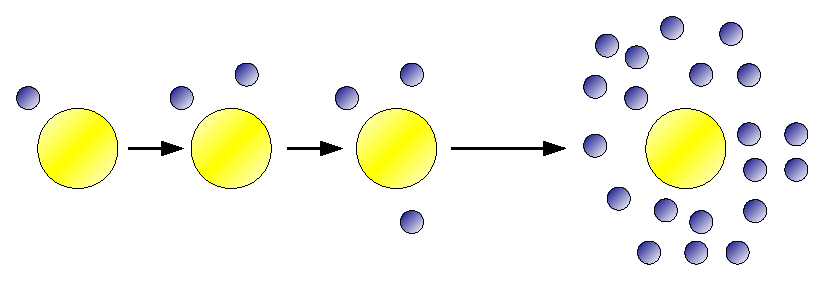
\includegraphics[scale=1]{Mikrosolvatace.eps}
\caption{Mikrosolvatace.}
\label{Mikrosolvatace}
\end{figure}

\item \textbf{QM/MM metody.} V~rámci tohoto přístupu studujeme část systému metodami kvantové chemie a část jednoduššími přístupy, s~použitím empirických potenciálů. Empirické potenciály popisují molekuly pomocí různých empirických vazebných příspěvků a interakce mezi molekulami je pak realizována elektrostatickými, repulzními a disperzními příspěvky.\footnote{Empirickým potenciálům se v~tomto textu nevěnujeme, čtenáře zde odkazujeme kupř. na text Petra Bouře na \url{http://hanicka.uochb.cas.cz/~bour/prednaska/prednaska.htm}}  Na kvantové úrovni řešíme většinou pouze ty nejdůležitější části systému, například aktivní centrum enzymu, okolí či roztok pak popisujeme metodami empirickými. Hamiltonián je pak dán jako


\begin{equation}
\hat{H} = \hat{H}_{QN} + \hat{H}_{MM} + \hat{H}_{QM/MM},
\label{rov:Sol-1}
\end{equation}

\noindent kde $\hat{H}_{QM}$ je hamiltonián pro molekulu rozpuštěné látky počítaný na kvantově-chemické úrovni, $\hat{H}_{MM}$ představuje empirický potenciál a $\hat{H}_{QM/MM}$ popisuje interakci mezi oběma částmi. V~nejběžnějším případě můžeme psát

\begin{equation}
\hat{H}_{QM/MM} = - \sum_i \sum_M \frac{q_M}{r_{iM}} + \sum_{\alpha} \sum_M \frac{Z_{\alpha} q_M}{R_{\alpha M}} + \sum_{\alpha} \sum_M 4 \epsilon_{\alpha M} \left[ \left( \frac{\sigma_{\alpha M}}{R_{\alpha M}} \right)^{12} - \left( \frac{\sigma_{\alpha M}}{R_{\alpha M}} \right)^6 \right],
\label{rov:Sol-2}
\end{equation}

\noindent
kde $q_M$ je náboj molekulárně-mechanického (MM) atomu $M$, $Z_{\alpha}$ je nábojové číslo kvan\-tově-mechanického (QM) atomu $\alpha$ a $\epsilon_{\alpha M}$ a $R_{\alpha M}$ jsou parametry Lennard-Jonesova potenciálu popisující repulzní a disperzní síly mezi kvantově-mechanickým atomem $\alpha$ a~mole\-ku\-lárně-mechanickými atomy $M$. Elektrony jdou označeny indexem $i$. Elektrony i~jádra rozpuštěné látky popsané na QM úrovni tedy \uv{cítí} parciální náboje MM atomů a k~tomu přidáváme repulzi a disperzní přitahování mezi QM a MM atomy. 

Díky QM/MM přístupu je tak možné studovat i velmi rozsáhlé systémy. O~důležitosti QM/MM metod svědčí i Nobelova cena za rok 2013 udělená právě za výzkumy v~tomto směru. 

\begin{figure} [htb]
\centering
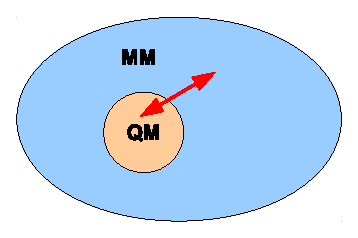
\includegraphics[scale=1]{QM_MM.eps}
\caption{Schéma strategie QM/MM.}
\label{obr:QM_MM}
\end{figure}


\item \textbf{Implicitní modely.} Představme si, že chceme vypočítat energii určitého iontu v~roztoku. Pro jednoduchost uvažujme ion kulovitého tvaru. Můžeme vypočítat energii iontu v~plynné fázi a připočítat solvatační energii. Ta je v~nejjednodušším případě dána Bornovou rovnicí, kdy solvatační energii vypočítáme z~rovnic klasické elektrostatiky jako rozdíl práce nutné k~nabití iontu ve vakuu a v~prostředí o~relativní permitivitě $\epsilon_r$


\begin{equation}
\Delta G_{sol} = - \frac{Z_i e^2}{8 \pi \epsilon_0 r_i} \left(1- \frac{1}{\epsilon_r} \right),
\label{rov:Sol-3}
\end{equation}

\noindent kde $r_i$ je poloměr příslušného iontu, $Z_i$ je nábojové číslo iontu a $\epsilon_0$  je permitivita vakua. Jde o~velmi přímočarou opravu na vliv solvatace, která ovšem nebere v~potaz některé složky solvatační energie. Tak kupříkladu zanedbává tzv. kavitační energii, tj. energii nutnou na vytvoření kavity, do které příslušný ion umístíme. Tuto veličinu můžeme odhadnout například z~hodnot povrchového napětí kapaliny, ve kterém molekulu solvatujeme. 

\begin{figure} [H]
\centering
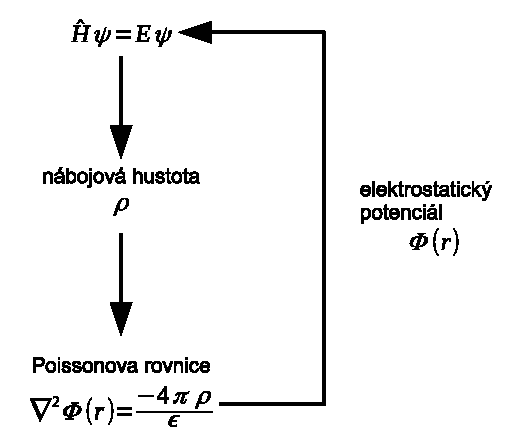
\includegraphics[scale=1]{SCRF_kolecko.eps}
\caption{Nástin algoritmu SCRF.}
\label{SCRF}
\end{figure}

\noindent Kromě toho předpokládáme, že elektronová struktura není solvatací ovlivněna. To ale není nutně splněno. Ion totiž polarizuje rozpouštědlo, které ho obklopuje, které ale zpětně působí svým polem na solvatovaný ion. Vytváří se tzv. reakční pole, ve kterém je ion umístěn. Korektní postup tak spočívá v~tom, že řešením Schr\"odingerovy rovnice vypočítáme elektrické pole generované naším iontem, v~tomto poli řešíme elektrostatické rovnice pro okolní roztok, získáme ono reakční pole a znovu a znovu opakujeme celý výpočet, dokud se již vlnová funkce ani reakční pole nemění (SCRF, z~angl. \textit{Self Consistent Reaction Field}). Tento přístup je pouze o~málo náročnější než výpočet ve vakuu a bývá proto často používán. Na druhou stranu je třeba být obezřetný, neboť model má svá dobře známá omezení.        

     


\end{itemize}